\chapter{Ergebnisse}
\label{ch:ergebnisse}

\section{Analyse des LSS- und LSR-Formates}

In der Online-Dokumetation von LimeSurvey gibt es zwar eine Sektion zum Thema Export und Export-Formate, der Abschnitt war aber bis vor kurzem leer.
Auch jetzt enthält das Kapitel nur eine oberflächliche Beschreibung der Formate, die genaue Struktur wird nicht erklärt.
Da diese allerdings benötigt wird, um eine Konvertierung vornehmen zu können, muss zunächst ermittelt werden, wie die .lss- und .lsr-Dateien genau aufgebaut sind.

Dies wurde bewerkstelligt, indem zunächst eine simple Umfrage erstellt wurde, welches eine Fragegruppe und drei Freitextfragen enthält.
Dafür wurde eine Instanz der LimeSurvey Community Edition benötigt, diese aufzusetzen war dank existierenden Docker-Compose-Dateien relativ simpel.

Nachdem die Struktur der Umfrage selbst, sowie der Fragegruppen so ermittelt werden konnte, wurden komplexere Dateien erstellt.
Diese enthielten zunächst Fragen mit festen Antwortmöglichkeiten, also vor allem Maskenfragen und Multiple Choice Fragen.
Nachdem so auch die Struktur der Antworten deutlich geworden war, wurden zuletzt die Matrixfragen eingebaut und die Struktur der Subfragen ermittelt.
Zuletzt wurden Anzeigebedingungen in die Umfragen eingebracht und deren Struktur ermittelt.

Das Ergebis dieser Analyse wird im Folgenden dargestellt (Es werden nicht alle existierenden Elemente angesprochen, sondern nur die für diese Arbeit relevanten, eine vollständige Auflistung kann im \cref{app:lss} gefunden werden):

\subsection{Grundlegende Struktur}

Das Wurzel-Element in LSS ist \el{document}.
Hier sind zuerst grundlegende Informationen wie die Datenbank-Version (443) und den Typ des Dokuments (\el{Survey}) enthalten.
Jedes der größeren direkten Kind-Elemente in \el{document} hat die gleiche Struktur.
Es gibt dort zwei Kind-Elemente, \el{fields} und \el{rows}. In \el{rows} gibt es \el{row} Elemente, welche die Informationen selbst in weiteren Elementen enthalten.
In \el{fields} gibt es \el{fieldname} Elemente, wobei es für jedes mögliche Kind-Element von \el{row} ein \el{fieldname} Element mit dem Namen des Kindelements als Text gibt.
In den Feldern werden also einmal alle Elemente genannt, die sich innerhalb einer Reihe befinden können.

\subsection{Fragegruppen}

Im Element \el{groups} werden Metadaten über Fragegruppen gesammelt, wie zum Beispiel die Gruppen-ID.
Diese sind aber auch in \el{group\_l10ns} enthalten, darüber hinaus finden sich auch noch weitere Inhalte wie Gruppenname und Sprache in diesem Element.
Daher werden später keine Informationen aus \el{groups} verwendet.
Ein \el{row} Element steht hier für eine Fragegruppe.

\subsection{Fragen}

Das Element \el{questions} enthält Metadaten über Fragen, wie die ID der Frage (\el{qid}), die ID der Gruppe, welche die Frage enthält (\el{gid}), einen Titel (\el{title}) und einen Buchstaben, welcher angibt, um was für einen Fragetyp aus \cref{met:q_types} es sich handelt (\el{type}).
Ein \el{row}-Element steht hier für eine Frage, pro \enquote{Haupt}-Frage in der Umfrage gibt es ein Element in \el{questions}.
\el{subquestions} enthält Subfragen von Arrays, Matrizen et cetera. Diese sind via das Feld \el{parent\_qid} an ein Element aus \el{questions} gekoppelt.
Auch in \el{subquestions} sind nur Metadaten enthalten, jede Subfrage hat, wie die \enquote{Haupt}-Fragen auch, eine Fragen-ID.

In \el{question\_l10ns} gibt es nun die eigentliche Frage in \el{question}, ein Element innerhalb einer Reihe.
Weiterhin gibt es mit \el{help} einen Hilfstext für die Frage, \el{language} gibt die Sprache des Fragetextes an.
Für jedes Element aus \el{question} und \el{subquestion} gibt es hier ein Element pro Sprache.
Referenziert werden diese mit der \el{qid}.

\el{question\_attributes} enthält Informationen über eine Frage wie ein Prä-/Suffix zu der Antwort, RegEx-Validations-Ausdrücke für die Antwort, Timings und Informationen zur Darstellung einer Frage (Textfeldbreite, Default-Antworten).
Für Fragen wie \el{Zahleneingabe} wird hier auch festgelegt, ob mit ganzen Zahlen oder Gleitkommazahlen geantwortet werden kann und ob die Antwort auf einen bestimmten Zahlenbereich begrenzt ist.

\subsection{Antwortmöglichkeiten}

Es gibt eine Reihe an Fragen, für die es eine Menge an vordefinierten Antworten gibt.
Diese sind entweder schon durch die Frage festgelegt, wie bei dem Fragetyp \el{5 Punkte Wahl} oder dem Typ \el{Geschlecht}, oder der Umfrage-Ersteller kann sie selber angeben.
Sind die Möglichkeiten schon durch den Typ festgelegt, werden die Antwortmöglichkeiten implizit ermittelt und nie konkret im LSS-Dokument niedergeschrieben.

Hat der Umfrage-Ersteller die Möglichkeiten selber festgelegt, werden diese in \el{answers} und \el{answer\_l10ns} gespeichert.
In \el{answers} gibt es dabei wieder Metadaten wie die ID der Frage, zu der die Möglichkeit gehört (\el{qid}), die ID der Antwortmöglichkeit (\el{aid}), und einen \el{code}, mit dem die Option später in den Antworten referenziert werden kann.
In \el{answer\_l10ns} hingegen gibt es den Antworttext in \el{answer}, eine \el{aid} zur Verknüpfung mit den Metadaten und die Sprache in \el{language}.
Für jedes Element aus \el{answers} gibt es pro Sprache ein Element in \el{answer\_l10ns}.

\subsection{Umfrage-Metadaten}
\label{a:survey_meta}

In \el{surveys} findet man Metadaten über die Umfrage, allerdings sind keine davon für die Konvertierung relevant.
Beispiele wären Daten darüber, ob Willkommenstexte angezeigt werden sollen oder ob IP-Adressen der Teilnehmer gespeichert werden sollen.
\el{surveyls\_languagesettings} enthält relevante Informationen wie die \el{surveyls\_id}, den Titel in \el{surveyls\_title} und eine Beschreibung der Umfrage (\el{surveyls\_description}).
\el{themes} und \el{themes\_inherited} enthalten Informationen über die visuelle Darstellung der Umfrage in LimeSurvey.

\subsection{LSR-Aufbau}
\label{a:lsr}

Auch für die Antworten wurde die gleiche Strategie wie für die Umfragestruktur verwendet.
Das sind die Ergebnisse:

Das Wurzel-Element ist wieder \el{Document}, zuerst gibt es wieder einige Metadaten wie der Typ des Dokuments (\el{Responses}), die Datenbank-Version und die Sprache.
Dann gibt es ein \el{responses} Element, welches dieselbe grundlegende Struktur wie die Elemente in der LSS-Datei besitzt.
Für jede Rückmeldung auf die Umfrage gibt es ein Element vom Typ \el{row}. Für den Rest der Arbeit wird eine Ausfüllung der Umfrage ebenfalls als \enquote{Rückmeldung}  bezeichnet werden.

Eine Rückmeldung enthält eine ID, ein Token, das Absendedatum, die Sprache, einen Seed und die Antworten.
Wenn ein Teilnehmer die Umfrage mehrmals ausfüllt, sind die IDs verschieden, die Tokens aber gleich.
Voraussetzung dafür ist aber, dass es eine feste, vorher festgelegte Liste von Teilnehmern gibt.
Gibt es diese nicht und jeder kann die Umfrage beantworten, wenn er den Link hat, gibt es kein \el{token} Element, sondern nur eine ID.

Bei den Antworten gibt es für jede Frage bzw. Subfrage ein Element mit folgendem Namensschema: 
\reg{\textunderscore\{Survey-ID\}X\{GID\}X\{QID\}\{SQID\}?\{ext\}?}
\noindent wobei \el{ext} folgendes sein kann: (\enquote{other}$\vert$\enquote{comment}).
Man kann bereits am Format sehen, dass es auch für die \enquote{other}- und Kommentar-Felder hier eine separate Antwort gibt.

\subsection{Erstellung eines XML-Schemas}
\label{an:xsd}
Da die Struktur der Umfrage nun bekannt ist, wird ein XML-Schema für das LSS-Format erstellt.
Das sorgt einerseits für eine wesentlich bessere Übersicht über den Aufbau, das kann für zukünftige Arbeit nützlich sein.
Andererseits lässt sich dieses Schema später verwenden, um zu überprüfen, ob es sich bei der Eingabedatei um eine valide LSS-Datei handelt.

\section{Mapping}

Da der Aufbau beider Formate nun bekannt ist, muss überlegt werden, wie man beide LimeSurvey-Formate auf ODM abbilden kann. Im Folgenden werden die verschiedenen Teile nacheinander abgehandelt und es wird erklärt, wie mit überschüssigen Elementen in ODM ungegangen wird.
Der Text wird dabei das Vorgehen beschreiben, die exakten Elementnamen können in den Grafiken nachgesehen werden.

\subsection{Dummy Elemente in ODM}

ODM besitzt mehr Möglichkeiten, die Abläufe einer Studie oder Umfrage darzustellen, da es als generisches Format natürlich mehr Einsatzzwecke abdecken soll, als das LSS-Format.
Dementsprechend gibt es mehrere Wege, LSS auf ODM abzubilden.

Durch die hier getroffenen Entscheidungen werden die Elemente \el{StudyEvent} und \el{GlobalVariables} überflüssig,	da es sich dabei um für eine Studie relevante Felder handelt, es soll aber nur eine Umfrage innerhalb einer Studie erstellt werden.

Da diese Elemente dennoch zwingend in ODM vorkommen müssen, werden die globalen Variablen leer gelassen oder mit Dummy-Werten befüllt und es wird ein \el{StudyEvent} erstellt, welches unabhängig von der Eingabe-Datei immer die gleichen Dummy-Werte hat.
Weiterhin wird die \el{OID} des \el{Study} Elements auch auf einen Dummy-Wert gesetzt, da wir hier ebenfalls kein Äquivalent in LSS haben.
Die \el{OID} der \el{MetaDataVersion} soll die Studien-ID behinhalten, da die Version der Metadaten die gesamte Umfrage enthält, es ergibt also Sinn, hier keinen Dummy-Wert einzusetzen sondern eine Referenz auf die Umfrage mit einzubringen.

\subsection{Umfrage-Eigenschaften}
\label{m:survey_meta}

Innerhalb unseres Dummy-\el{StudyEvent's} gibt es nun ein Formular, dieses wird die Umfrage repräsentieren (siehe \cref{fig:props}).
Das \el{Repeating} Attribut wird auf \enquote{Yes} gesetzt, da die Umfrage potentiell mehrfach pro Teilnehmer ausgefüllt werden kann, wenn es eine feste Liste an Teilnehmern gibt.
Da das Formular die Umfrage repräsentiert, sollen sie dieselbe ID nutzen, als \el{Name} wird der Titel der Umfrage gesetzt. Die Beschreibung wird ebenfalls in das Formular übernommen.

\subsection{Fragegruppen}
\label{m:qg}
Fragegruppen in LimeSurvey sind fast äquivalent zu \el{ItemGroup's} in ODM, für diese Abbildung sind sie isomorph.
Entsprechend wird für jede Fragegruppe eine \el{ItemGroupDef} erstellt, die ID wird direkt in ODM übernommen, der Titel wird als Name verwendet, die Beschreibung kann ebenfalls direkt übernommen werden (\cref{fig:groups}).
Das Attribut \el{Repeating} wird auf \enquote{No} gesetzt. %TODO: Erklären
Entsprechende Referenzen auf die Fragegruppen werden zum Formular hinzugefügt.

\begin{figure}[h]
	\makebox[\linewidth][c]{%
		\begin{subfigure}[b]{.6\textwidth}
			\centering
			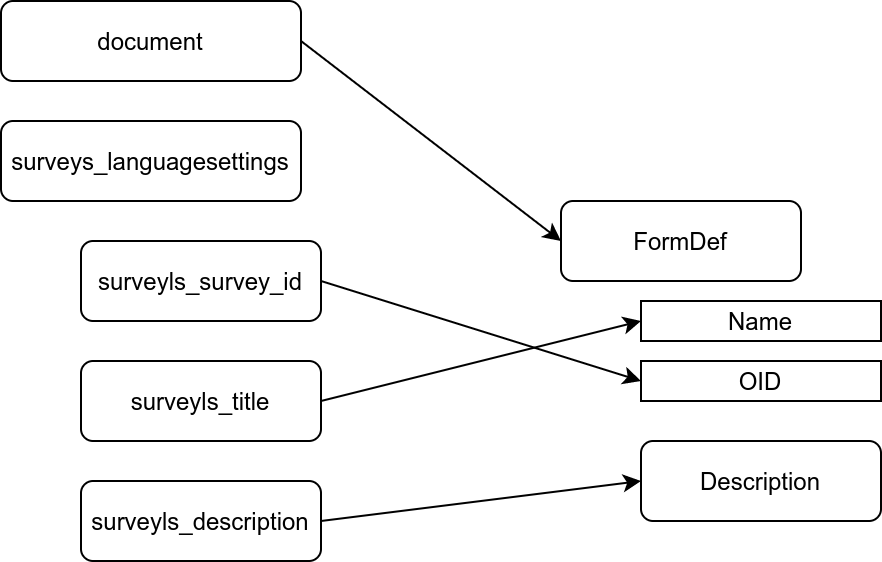
\includegraphics[width=.95\textwidth]{./img/m_survey_props.png}
			\caption{Mapping der Umfrage-Eigenschaften}
			\label{fig:props}
		\end{subfigure}%
		\begin{subfigure}[b]{.6\textwidth}
			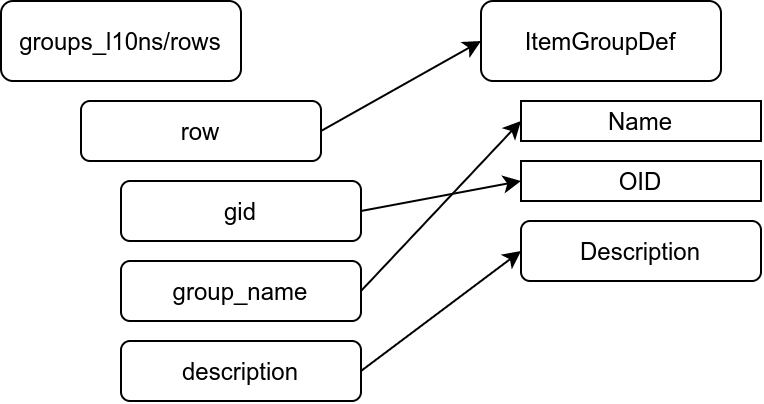
\includegraphics[width=.95\textwidth]{./img/m_groups.png}
			\caption{Mapping der Fragegruppen}
			\label{fig:groups}
		\end{subfigure}%
		}
		\caption{Diagramme für Fragegruppen und Umfragen}
\end{figure}

\subsection{Fragen}

Fragen, welche keine Subfragen besitzen, werden direkt in ODM übernommen.
Wie schon bei den Fragegruppen wird die ID übernommen und der Titel wird zum Namen.
Der Fragetext aus \el{question} wird in ODM bei \el{Question/TranslatedText} der Fragedefinition eingetragen. Die Sprache wird im Attribut \el{lang} eingetragen (siehe \cref{fig:questions}).
Der Hilfstext der Frage wird zur Beschreibung in ODM.
Die Angabe, ob eine Frage verpflichtend ist, kann ebenfalls übernommen werden, allerdings wird diese in ODM in der Fragen-Referenz eingetragen, nicht in der Definition.

In ODM gibt es keine Subfragen, dementsprechend muss eine Frage in LimeSurvey potentiell in mehrere Fragen, eine pro Subfrage, umgewandelt werden, damit diese in ODM eingefügt werden können.
Daher muss jeder Fragetyp aus LimeSurvey einzeln behandelt werden, wobei sich die benötigten Arbeitsschritte teils überschneiden.
Auch sind die Behandlungen für mehrere Fragetypen identisch.
Zum Beispiel werden die Fragetexte der Hauptfrage und der Subfrage konkateniert, um so eine neue Frage  zu formulieren.
Für die Festlegung der \el{OID} von Subfragen wird die \el{qid} der Hauptfrage mit dem Titel der Subfrage konkateniert.
Gründe dafür werden in \cref{im:ans} dargelegt.
Im folgenden werden alle Behandlungen erklärt, mit einer Angabe, für welche Fragetypen diese genutzt werden.

\begin{figure}[h]
	\centering
	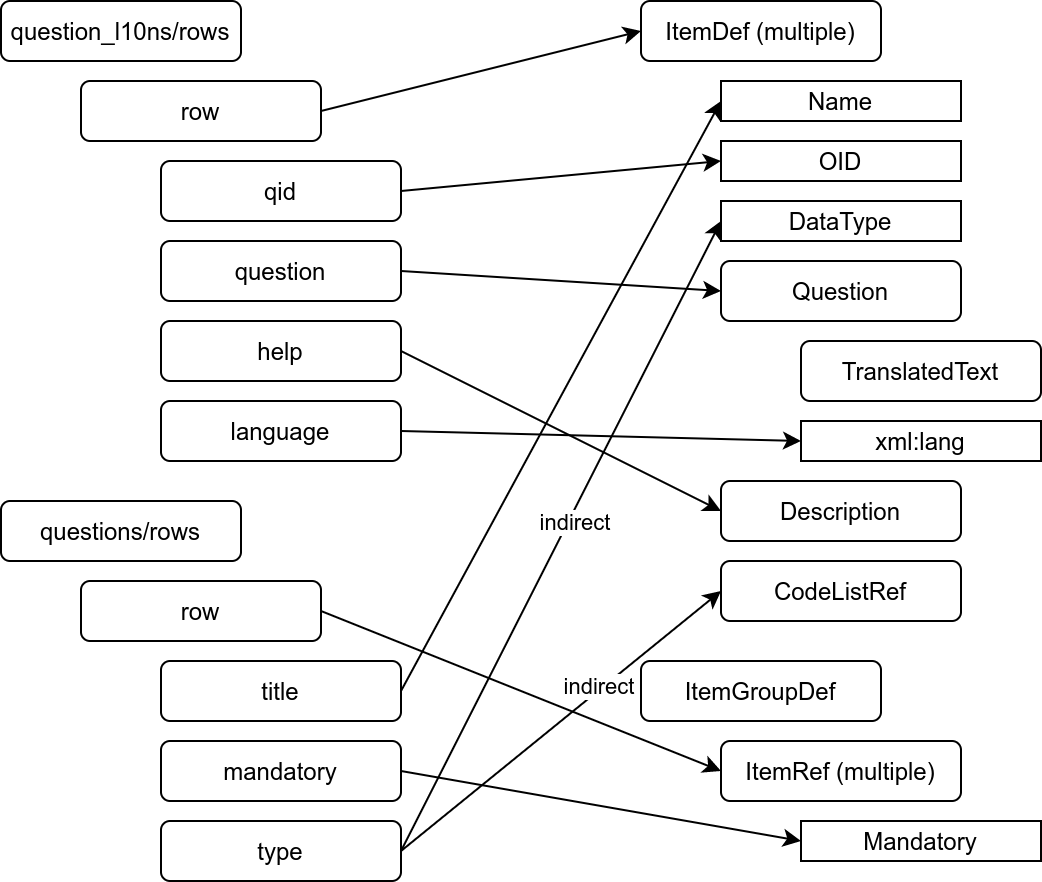
\includegraphics[width=.95\textwidth]{./img/m_questions.png}
	\caption{Mapping der Fragen}
	\label{fig:questions}
\end{figure}

\subsubsection{Einfachauswahl}
\label{e:sc}

Hier werden die Fragen 1:1 abgebildet, die Antwortmöglichkeiten werden in einer \el{CodeList} gespeichert.
Für den Typ \el{Liste mit Kommentar} wird eine weitere Frage hinzugefügt, deren \el{OID} die \el{qid} der Frage ist, allerdings wird noch \enquote{comment} angehangen.
An den Fragetext wird ebenfalls das gleiche angehangen.
Bei dem Bild der \el{Image-Select-List} besteht das Problem, dass dieses nur mittels Link zum Bild auf dem LimeSurvey-Server eingebettet ist.
Beim Übertragen der Fragen ist somit auch nur dieser Link enthalten.

\subsubsection{Matrix}

Für die Matrizen mit Zahlen- oder Freitextantworten wird eine Frage pro Zelle der Matrix hinzugefügt.
Für alle weiteren Typen dieser Kategorie bis auf die \el{Dual Matrix} wird eine Frage pro Subfrage hinzugefügt, die gleiche Liste an Antwortmöglichkeiten wird für jede Subfrage verwendet.
Die \el{Dual Matrix} wird behandelt, als würde die gleiche Frage zwei Mal mit unterschiedlichen Antwortmöglichkeiten gestellt.

\subsubsection{Multiple Choice}

Hier wird eine Frage pro Subfrage hinzugefügt, gibt es Kommentare, wird noch eine entsprechende Kommentar-Frage pro Subfrage eingefügt.
Das Bild beim Typ \el{Image Select} wird wie schon bei der Einfachauswahl nur auf Umwegen übernommen.

\subsubsection{Textfragen}

Hier wird der Fragetext wie oben erklärt übertragen, als \el{DataType}-Attribut in \el{ItemDef} wird \enquote{string} gesetzt.
Das funktioniert für alle drei Freitextfragetypen, kurz, lang und riesig so.
Im Falle von \el{Mehrere Texte} und \el{Input on Demand} wird wieder eine Frage pro Subfrage genutzt.
\el{Browser Detect} wird nicht gemappt. Für Details siehe \cref{d:leave}.

\subsubsection{Maskenfragen}

Für den Typ \el{Datum/Zeit} wird der \el{DataType} auf \enquote{datetime} gesetzt.
Für \el{Zahleneingabe} wird der \el{DataType} auf \enquote{float} gesetzt, außer die Option \enquote{Nur Integers} ist angewählt, dann wird stattdessen \enquote{integer} genutzt.
Für \el{Mehrfache Zahlen} wird wieder eine Frage pro Subfrage erstellt.
Für beide Zahlen-Fragen werden Frageattribute, wie den maximalen oder minimalen Antwort-Wert als \el{RangeCheck} übernommen.

Es gibt mehrere Typen, bei denen es feste Antwortmöglichkeiten gibt und daher eine CodeList implizit aus dem Typ erstellt wird:
\el{Ja/Nein}, \el{Geschlecht}.
Beim Typ \el{Gleichung} handelt es sich nicht um eine Frage, er wird nicht gemappt (siehe \cref{d:leave}).
\el{Ranking}, \el{Textanzeige}, \el{Dateiupload} und \el{Sprachumschaltung} werden nicht gemappt. Für weitere Details siehe \cref{d:leave}.

\subsection{Antwortmöglichkeiten}

\begin{figure}[h]
	\centering
	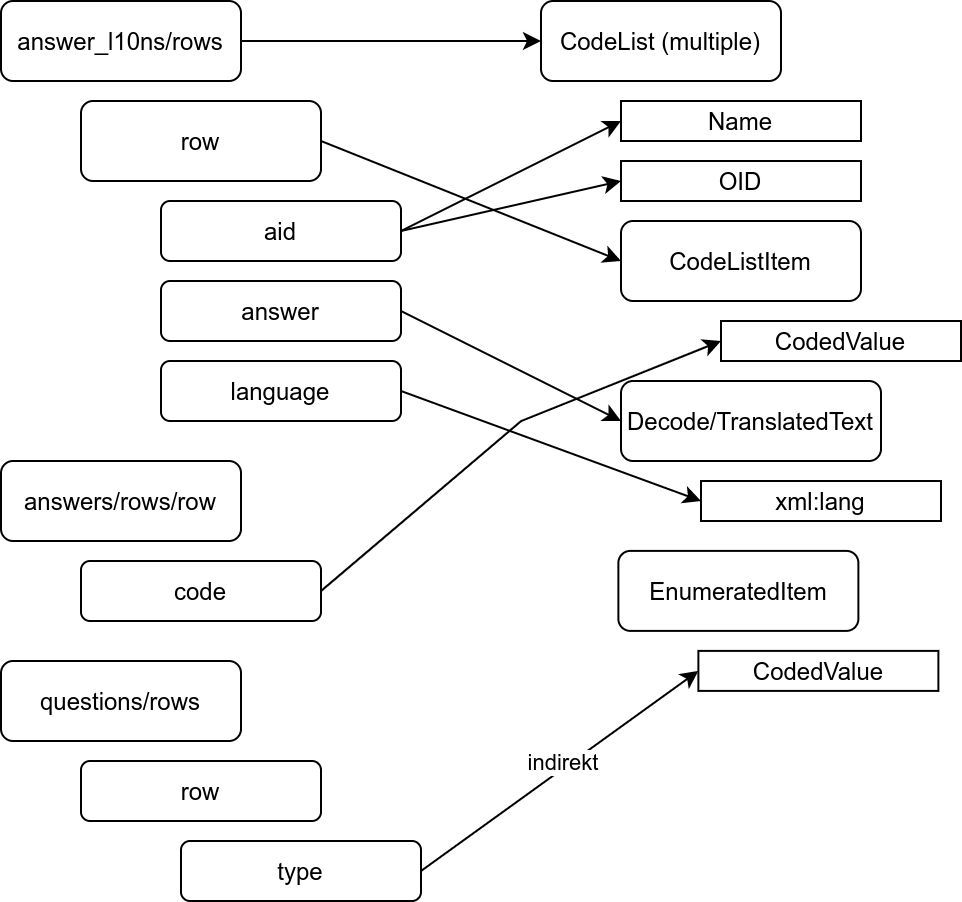
\includegraphics[width=.9\textwidth]{./img/m_answers.png}
	\caption{Mapping der Antwortmöglichkeiten}
	\label{fig:ans}
\end{figure}

Grundsätzlich wird jedes Mal, wenn es eine vordefinierte Liste an Antwort- möglichkeiten gibt, eine CodeList genutzt, um diese Liste in ODM darzustellen.
Das kann man in \cref{fig:ans} sehen.
Für die Fragen, wo man mit 1 bis 5 oder 1 bis 10 antworten kann, wird eine simple Liste genutzt, für alle weiteren Fragen eine komplexe Liste.
Das liegt unter anderem daran, dass LimeSurvey fast alle Antworten mit einem Buchstaben darstellt und die tatsächlichen Antworten aus mindestens einem Wort bestehen.
So werden komplexere Umwandlungen vermieden und die existierende Struktur wird übernommen.
Für selbstdefinierte Antwortmöglichkeiten ist ohnehin eine komplexe Liste notwendig, da der Ersteller der Umfrage beliebige Kombinationen für Code und Antwort definieren kann.

\subsection{Antworten}

\begin{figure}[h]
	\centering
	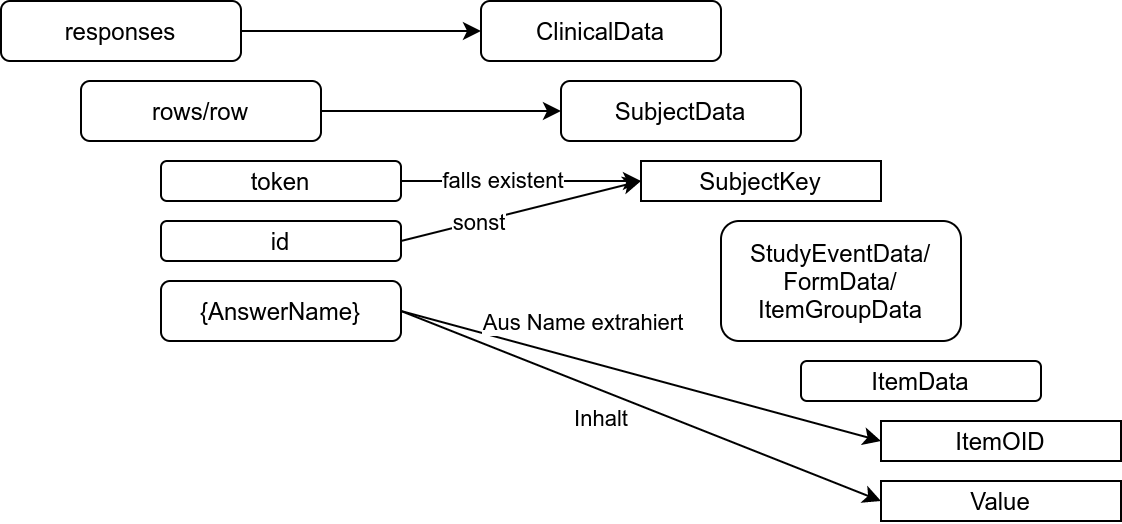
\includegraphics[width=1\textwidth]{./img/m_lsr.png}
	\caption{Mapping des LSR-Formates}
	\label{fig:m:lsr}
\end{figure}

Die Antworten werden in die klinischen Daten von ODM übertragen, die Abbildung ist in \cref{fig:m:lsr} zu sehen.
Da es in LimeSurvey keine Sortierung nach den Teilnehmern gibt, wird die \el{SubjectData} immer zustätzlich eingefügt, falls notwendig.
Als \el{SubjectOID} wird ein Token, falls es ein solches gibt, verwendet. Das liegt daran, dass ein Token pro Teilnehmer eindeutig ist, während es pro Teilnehmer mehrere IDs in LimeSurvey geben kann.
Gibt es kein Token, wird die ID aus LimeSurvey als ID on ODM genutzt.
Ein passender \el{RepeatKey} wird ebenfalls festgelegt, sodass verschiedene Rückmeldungen auf die Umfrage durch den gleichen Teilnehmer unterschieden werden können.

Als \el{StudyOID}- und \el{MetaDataVersionOID}-Attribute der \el{ClinicalData} werden die entsprechenden OIDs referenziert.
Für die OIDs des \el{StudyEvent's} und des Formulars werden die bereits erstellten Werte eingetragen.
Da eine Reihe einer Ausfüllung der Umfrage entspricht, wird die Reihe auf die Daten eines Formulars abgebildet.
Als ID der Fragegruppe wird die \el{gid} gesetzt.
Als \el{ItemOID} des \el{ItemData} Elements wird ein Teil des Elementnamens genutzt, nämlich \enquote{\{qid\}\{sqid\}\{ext\}}, in \el{Value} wird der Text des Elements eingetragen.
Da die OIDs der Fragen vorher bereits so gewählt wurden, dass sie mit dieser Stuktur übereinstimmen, gibt es bereits funktionierende Referenzen, ohne weitere Umwandlungen vornehmen zu müssen.

\subsection{Themes und Frageattribute}

Die Themes werden nicht in ODM übernommen. Begründungen dazu gibt es in der Diskussion (\cref{d:themes}).
Auch von den Frageattributen werden keine übernommen, solange sie im Mapping nicht explizit erwähnt wurden, da die meisten der visuellen Darstellung dienen.

\section{Implementierung: LSA $\rightarrow$ ODM}
\label{im:lsa2odm}

\subsection{Java}

Ein Konverter zwischen XML-Dokumenten kann in vielen verschiedenen Programmiersprachen geschrieben werden.
Java bietet sich dabei aus verschiedenen Gründen an.
Einerseits gibt es viele Bibliotheken für Java, welche das Bearbeiten von XML stark vereinfachen, sie können fast alles, was man brauchen könnte, um die Aufgabe zu erfüllen.
Darunter sind zum Beispiel Validatoren, die XSD 1.1 unterstützen und Parser, welche mit mehreren Attributen in einem Element umgehen können.
Andererseits wird die Sprache bereits viel am IMI genutzt, der Konverter kann also sehr leicht als JAR in andere Programme eingebunden und von dort aus genutzt werden.

\begin{figure}[h]
	\centering
	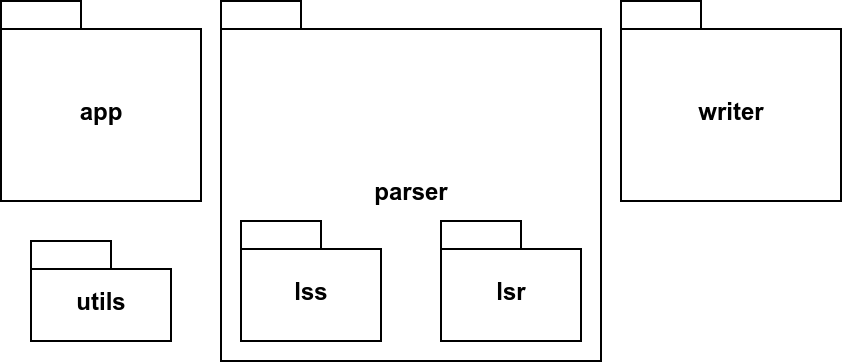
\includegraphics[width=.60\textwidth]{./img/i_package.png}
	\caption{Paketdiagramm für lsa2odm}
	\label{fig:package}
\end{figure}

\subsection{Programmaufbau}

Das Programm trägt den Namen \enquote{lsa2odm} und besteht aus vier Paketen, \jv{app}, \jv{utils}, \jv{parser} und \jv{writer}, wobei \jv{parser} in zwei weitere Pakete aufgeteilt ist, \jv{lss} und \jv{lsr} (siehe \cref{fig:package}).
In \jv{app} befindet sich die Klasse \jv{App}, welche die \jv{main}-Methode enthält.
Diese leitet die Parameter an die statische Methode \jv{convert} der Klasse \jv{LsaConverter} weiter.

\subsection{Eingabe}

Das Programm erwartet entweder eine oder zwei Eingaben. Der erste Parameter muss dabei der Pfad zum LSA-Archiv sein, der zweite, optionale Parameter ist dabei ein Pfad, wo die ODM-Datei am Ende geschrieben werden soll.
Die entpackten Dateien werden auch zwischenzeitig an diesem Pfad abgelegt.
Anschließend wird der erste Parameter auf Validität getestet.
Zu diesem Zweck dient der reguläre Ausdruck:
\reg{\textasciicircum/?[.*/]*(.*?)\textbackslash\textbackslash.lsa\$}
\noindent Ist der Parameter ein gültiger Pfad zu einer Eingabedatei, wird \jv{unzipFile} auferufen.
Die Funktion beinhaltet generischen Code, welcher ein Zip-Archiv entpackt.
Wenn die Funktion fertig ist, kann man auf alle benötigten Dateien zugreifen und es kann mit den nächsten Aufgaben weiter gemacht werden.

\subsection{Properties}

Es gibt eine Reihe an Strings, welche im Programm gesetzt werden, besonders die Namen der Dummy-Elemente.
Aber auch Suffixe für manche Namen oder der Name der IMI-Syntax ist nicht festgelegt.
Daher sollen all diese Dinge von außerhalb des Codes geändert werden können.
Gibt es noch keine, wird eine Properties-Datei erstellt, welche all diese Informationen beinhaltet.

\subsection{XSD-Validierung}


Das in \cref{an:xsd} erstellte Schema wird nun genutzt, um zu überprüfen, ob die Eingabedatei valide ist.
Dazu wird der Validator aus \jv{utils} (\cref{fig:utils}) verwendet.
Das Ergebnis der Prüfung wird dem Nutzer angezeigt, allerdings ist es nicht bindend, auch eine invalide Datei wird konvertiert.
Das liegt vor allem daran, dass sich das Format schnell ändern kann, mehr dazu in \cref{d:version}.
Da diese Änderungen aber oft klein sind, besteht eine hohe Chance, dass der Konverter den Großteil des Dokumentes dennoch verarbeiten kann.
Der Anwender bekommt dennoch die Information, dass der Konverter potentiell nicht mit dieser LimeSurvey-Version funktioniert.

\subsection{Parsing der LimeSurvey Struktur}

Zuerst wird eine Instanz der Klasse \jv{LssParser} mit der entsprechenden LSS-Datei erstellt (\cref{fig:lss2}).
Die Klasse \jv{Survey} dient zum speichern aller gesammelten Informationen, alle für die ODM-Datei benötigten Daten werden hier abgelegt, das Objekt wird später weitergegeben.

Zunächst werden die drei in \cref{a:survey_meta} angesrochenen Elemente mit Metadaten der Studie in \jv{survey} übernommen, wie man in \cref{fig:lss_im} sehen kann.
Dann werden die Fragegruppen übernommen, hierbei werden alle für das Mapping relevanten Informationen, welche in \cref{m:qg} aufgelistet werden, gespeichert.

\begin{figure}[h]
	\begin{enumerate}
		\item Lese Datei ein
		\item Lese Umfrage-Eigenschaften aus
		\item Für jede Fragegruppe:
			\begin{enumerate}
				\item Erstelle ein neues Fragegruppen-Objekt mit den Werten der Gruppe
			\end{enumerate}
		\item Für jede Frage:
			\begin{enumerate}
				\item Erstelle ein neues Frage-Objekt aus den Werten der Frage
				\item Füge Bedingungen hinzu, welche zur Frage gehören
				\item Wähle passende Behandlung in Abhängigkeit vom Fragetyp
			\end{enumerate}
	\end{enumerate}
	\caption{Ablauf des LSS-Parsings}
	\label{fig:lss_im}
\end{figure}

\subsubsection{Parsing der Fragen}
\label{im:q}

Als nächstes werden die Fragen in \jv{survey} übernommen. Dabei werden diese bereits gemäß des Mappings umgewandelt.
Das wird gemacht, um die Gesamtstruktur so früh wie möglich zu simplifizieren und nicht für jede Frage eine gesonderte Klasse erstellen zu müssen.
Da sich viele Fragen im Aufbau stark ähneln, ist dies ein simpler und schneller Weg, das Ziel zu erreichen.
Am Ende dieser Verarbeitung soll es noch fünf Fragetypen geben:

\begin{enumerate}[font=\bfseries, leftmargin=0.5cm]
\item[T] Eine Frage, auf die mit einem Freitext geantwortet werden kann
\item[N] Bei dieser Frage muss mit einer Zahl im float-Format geantwortet werden
\item[I] Bei dieser Frage muss mit einer Zahl im integer-Format geantwortet werden
\item[A] Bei dieser Frage muss aus einer vordefinierten Liste an Antwortmöglichkeiten gewählt werden
\item[D] Diese Frage hat ein Datum und eine Uhrzeit als Antwort
\end{enumerate}

Zuerst wird eine Liste aller \el{row} Elemente des Frage-Elements erstellt, durch welche im Anschluss iteriert wird.
Die Klasse \jv{Question} soll alle Informationen über eine Frage speichern, entsprechend wird diese genutzt, um die Informationen jeder Reihe zu speichern.
Eine Liste der Daten ist in \cref{im:fig:lss} zu sehen.
Nicht in jedem Fall wird diese Frage auch zur Umfrage hinzugefügt, wenn es sich zum Beispiel um eine Matrix-Frage handelt, wird diese Instanz nur zum Erstellen neuer Fragen genutzt.
Dann werden potentiell existierende Bedingungen hinzugefügt, dieser Vorgang wird in \cref{im:cond} beschrieben.

Anschließend gibt es ein \jv{switch}-Statement, welches einen passenden Weg zum Parsen der Frage abhängig vom Typ ausführt.

\subsubsection{Textfragen}
Für Textfragen wird hier nur der Typ geändert, sodass alle Arten von Textfragen \enquote{T} als Typ haben.

\subsubsection{Datum/Zeit}
Bei Datum/Zeit-Fragen wird die \el{qid} zu einer Liste hinzugefügt, welche später in \cref{im:ans} gebraucht wird.

\subsubsection{Numerische Eingaben}
Wenn es sich um eine Frage mit numerischer Antwort handelt, wird geprüft, ob die Antwort nur ganzzahlige Werte enthalten darf. In dem Fall wird der Typ auf \enquote{I} gesetzt. 
Dann wird überprüft, ob es Minimal- und Maximalwerte für die Antwort gibt, wenn ja werden die entsprechenden Werte in der Frage-Klasse gesetzt.
Zur Überprüfung wird das entsprechende Attribut aus \el{question\_attributes} ausgelesen.

\subsubsection{Listen}
Handelt es sich um eine Frage vom Typ \el{Liste mit Kommentar}, wird zuerst eine weitere Frage hinzugefügt, welche den Kommentar speichern soll.
Dann wird mit der Behandlung für die anderen \el{Listen}-Fragen fortgefahren.
Bei selbiger wird geschaut, ob die Option für \jv{Anderes} aktiviert ist, wenn ja, wird auch dafür eine Frage hinzugefügt.
Dann wird eine Liste mit Antwortmöglichkeiten an die eigentliche Frage angehangen und selbige wird hinzugefügt.

\subsubsection{Restliche Einfachauswahl}
Für die Fragetypen \el{Fünf Punkte Auswahl}, \el{Ja/Nein} und \el{Geschlecht} wird der Typ geändert und eine entsprechende Antwort-Liste mittels der dafür erstellten Hilfsfunktionen generiert.

\subsubsection{Multiple Antworten}

Wird nach Zahlen verlangt, werden erst potentielle Constraints ermittelt und hinzugefügt, dann wird der Typ angepasst, je nach Gleitkomma- oder Ganzzahl-Antworten.
Dann wird bei beiden die Funktion \jv{addSubquestions} aufgerufen.
Diese sucht die IDs aller Subfragen und fügt dann entsprechende Kopien der Hauptfrage ein, Änderungen werden wie oben beschrieben durchgeführt.

\subsubsection{Duale Skalen}

Geht es um diesen Typ, werden erst beide Listen mit Antworten angelegt, dann wird die Funktion \jv{addSubquestionsWithCL} zwei Mal aufgerufen, einmal mit jeder Skala.
Beim ersten Mal wird \enquote{-0} an die Frage-ID angehangen, beim zweiten Mal \enquote{-1}.

\subsubsection{Matrizen (Text, Numerisch)}

In beiden Fällen werden hier die Antwortmöglichkeiten auf den Achsen gesammelt, dann wird für jede Kombination eine neue Frage erstellt, der Inhalt wird angepasst.

Dabei wird die Frage-ID wie folgt aufgebaut: \enquote{\{Parent\_QID\} + \{Title(y-Axis)\}\_\{Title(x-Axis)\}}.

\subsubsection{Arrays}

Für alle Array-Fragen wird die Funktion \jv{addSubquestionWithCL} aufgerufen, die Liste an Antworten, deren Name un der Datentyp wird jeweils angepasst.

\subsubsection{Mehrfachauswahl}

Hier werden auch alle Subfragen mit einer Antwortliste eingefügt, die Liste enthält \enquote{Y} für Ja und \enquote{} für Nein.
Dann wird noch eine potentielle \jv{Anderes}-Frage eingefügt.
Hat die Auswahl noch Kommentare, wird eine spezielle Methode aufgerufen.
Diese hat fast den gleichen Inhalt, wie die Methode für Subfragen mit einer Antwortliste, allerdings wird noch ein Kommentar für jede Frage eingefügt.
Eine passende Bedingung wird auch eingefügt, sodass die Kommentar-Frage nur angezeigt wird, wenn die Möglichkeit auch ausgewählt wurde.


\subsubsection{Parsing der Anzeige-Bedingungen}
\label{im:cond}

Da die Bedingungen innerhalb des LSS-Formates ohnehin als Elemente gespeichert werden und nicht als ExpressionScript, ergibt es mehr Sinn, diese nicht wieder in ExpressionScript umzuwandeln, sondern direkt in die Syntax des IMI.
Die in LimeSurvey mit ExpressionScript formulierten Bedingungen geben an, wann eine Frage angezeigt werden soll.
Die in ODM definierten Bedingungen müssen zu \enquote{True} evaluieren, wenn eine Frage nicht angezeigt werden soll.
Der fertige Ausruck muss am Ende also negiert werden.
Dann werden alle Bedingungen rausgesucht, welche zur \el{qid} gehören.
Diese werden durch ein logisches \enquote{Und} verknüpft.
Der Ablauf ist in \cref{fig:cond_im}

\begin{figure}[h]
	\begin{enumerate}
		\item Erstelle eine neue Zeichenkette für die Gesamtbedingung
		\item Für Jede Bedingung der Frage:
			\begin{enumerate}
				\item Erstelle eine neue Zeichenkette für die Bedingung
				\item Finde die QID und GID der referenzierten Frage und erstelle einen Pfad in IMI-Syntax
				\item Wenn es sich um eine RegEx-Bedingung handelt:
					\begin{enumerate}
						\item Setze die Bedingung auf \enquote{MATCH(\{Wert\}, \{Pfad\})} 
					\end{enumerate}
				\item Sonst: Setze die Bedingung auf \enquote{(\{Pfad\}\{OP\}\{Wert\})}
				\item Füge die Bedingung zur Gesamtbedingung hinzu
				\item Falls dies nicht die letzte Bedingung ist, füge \enquote{AND} zur Gesamtbedingung hinzu
			\end{enumerate}
	\end{enumerate}
	\caption{Das Verarbeiten der Bedingungen einer Frage}
	\label{fig:cond_im}
\end{figure}

Die Frage aus \el{cfieldname} wird mittels des regulären Ausdrucks
\reg{\textasciicircum\textbackslash\textbackslash d+X(\textbackslash\textbackslash d+)X(.+?)\$}
\noindent so verarbeitet, dass wir die darin enthaltene \el{gid} und \el{qid} der Frage enthalten.
Mit diesen, der Dummy-ID für das \jv{StudyEvent} und der Umfragen-ID wird dann ein Pfad gemäß der IMI-Syntax erstellt.

Handelt es sich nicht um einen regulären Ausdruck, der als Operator genutzt wird, werden folgende drei Teile in dieser Reihenfolge aneinander gehangen: 
\reg{\{PATH\} \{OPERATOR\} \{VALUE\}}
\noindent wobei das Element \el{method} den Operator enthält und \el{value} den Wert. \jv{PATH} ist der vorher erstellte Pfad.

Handelt es sich um einen regulären Ausdruck, wird das führende Leerzeichen entfernt und die Bedingung in folgender Form aufgeschrieben:
\reg{MATCH(\{REGEX\}, \{PATH\})}

Soll eine Antwort leer bleiben, wird \enquote{NULL} als Wert verwendet.
Sowohl beim Vorgehen für reguläre Ausdrücke und für leere Antworten handelt es sich nicht um einen Teil der IMI-Syntax, weiteres dazu in \cref{d:imi}.

Abschließend wird der Bedingung eine OID der Form \el{\{qid\}\{ex\}} gegeben, wobei \el{ex} in der Properties-Datei festgelegt werden kann.
Die OID wird auch in der Frage eingetragen, damit man später eine Referenz auf die Bedingung hat.

\subsection{Parsing der LimeSurvey Antworten}
\label{im:ans}

In \cref{alg:lsr} sieht man den Plan, wie die Antworten verarbeitet werden sollen.
Die Klasse \jv{LsrParser}, zusammen mit den Klassen \jv{Response} für eine Rückmeldung und \jv{Answer} für eine Antwort wurden dafür in Java erstellt.
Zuerst wird ein neuer SAXReader erstellt, welcher die LSR-Datei in eine Instanz der Klasse \jv{Document} einliest.
Selbige wird dann in \jv{parseAnswers} weiterverwendet.

\begin{figure}[h]
	\begin{enumerate}
		\item Erstelle ein neues Dokument
		\item Für jede Rückmeldung:

			\begin{enumerate}
				\item Erstelle eine neue Rückmeldung
				\item Setze ID auf das \el{Token}, wenn es das nicht gibt, setze sie auf die \el{ID}
				\item Für jede Antwort:

					\begin{enumerate}
							\item Wenn die Antwort nicht leer ist, füge sie zur Rückmeldung hinzu
					\end{enumerate}
			\end{enumerate}
	\end{enumerate}
	\caption{Das Vorgehen beim Verarbeiten der Antworten in Pseudocode}
	\label{alg:lsr}
\end{figure}

In den Reihen des \el{responses} Elements gibt es eine Reihe pro Rückmeldung auf den Fragebogen.
Die Klasse \jv{Response} dient zum Speichern einer Reihe, daher werden Instanzen erstellt, um alle Informationen der LSR-Datei zu übertragen.
Als nächstes wird über alle Kind-Elemente der Reihe iteriert und es wird nach Antworten gesucht.
Wie in \cref{a:lsr} zu sehen, sind nicht alle Kind-Elemente auch Antworten, daher muss gefiltert werden.
Antworten sind an der Struktur des Element-Namens zu erkennen, diese ist in \cref{a:lsr} beschrieben.
Da sich die Struktur bis auf den führenden Unterstrich nicht von dem Text des Elements \el{cfieldname} aus \cref{im:cond} unterscheidet, können wir fast den gleichen regulären Ausdruck \enquote{\textasciicircum\textunderscore\textbackslash\textbackslash d+X(\textbackslash\textbackslash d+)X(.+?)\$} verwenden, um pasende Elemente zu finden und mittels der Capture Groups die \jv{gid} und \jv{qid} zu erhalten.

Dann wird geprüft, ob die Antwort leer ist, in dem Fall wird sie ignoriert.
Ist sie nicht leer, wird geschaut, ob es sich um eine \el{Datum/Zeit} Frage handelt, dazu wird die in \cref{im:q} erstellte Liste genutzt. Handelt es sich um so eine Frage, wird das Leerzeichen, welches Datum und Uhrzeit trennt, durch ein \enquote{T} ersetzt.
Dies ist notwendig, damit das Format dem Datentyp \enquote{xsd:dateTime} entspricht, welcher später gefordert wird.
Anschließend wird eine neue Instanz der Klasse \jv{Answer} erstellt, diese soll die Antwort auf eine Frage sichern.
Befüllt wird sie mit den vorher gewonnenen Informationen über die Frage.

Schließlich wird die Antwort mittels der Methode \jv{addToAnswers} zum \jv{answers}-Objekt der Umfrage hinzugefügt.
Diese Methode sortiert die Antwort dabei passend ein, sodass am Ende alle Antworten zu Fragen aus der gleichen Fragegruppe in einer Liste sind.

Dann wird die \jv{Response} in die ensprechende Liste hinzugefügt.

\subsection{Ausgabe als ODM-Datei}

Mittels der Klasse \jv{ODMWriter} soll eine neue ODM-Datei erstellt werden. Der Konstruktor nimmt dabei das beim Parsing erstellte \jv{Survey}-Objekt entgegen, welches alle aus LimeSurvey gewonnenen Daten enthält. %TODO: LS oder LSS?
Das Erstellen einer ODM-Datei aus einer Umfrage ist dabei mit nur einer Methode möglich.

\begin{figure}[t]
	\begin{enumerate}
		\item Erstelle ein neues Dokument
		\item Füge das Wurzelelement samt Attributen ein
		\item Füge eine neue Studie, globale Variablen und eine Version der Metadaten ein
		\item Befülle die Metadaten mit einem Protokoll, einem Studien-Event und einem Formular
		\item Für jede Fragegruppe:
			\begin{enumerate}
				\item Füge eine Referenz zum Formular hinzu
				\item Ergänze die Definitionen in den Metadaten
			\end{enumerate}
		\item Für jede Frage:
			\begin{enumerate}
				\item Füge eine Referenz zur passenden Fragegruppe hinzu
				\item Ergänze die Definitionen in den Metadaten
				\item Falls es eine Liste an Antwortmöglichkeiten gibt:
					\begin{enumerate}
						\item Füge diese zu dem Metadaten hinzu
					\end{enumerate}
			\end{enumerate}
		\item Füge das Element für die klinischen Daten zum Wurzelelement hinzu
	\end{enumerate}
	\caption{Prozedere bei der Erstellung des ODM-Dokuments}
	\label{alg:odm}
\end{figure}

\subsubsection{Studienstruktur}

Zuerst wird das Wurzelelement namens \el{ODM} erstellt.
Dabei werden auch Attribute hinzugefügt, darunter die Schema- und Namespace-URLs. Benötigt werden weiterhin ein Dateityp, eine OID für die Datei und der Erstellungszeitpunkt.
Als Dateityp wird hier \jv{Snapshot} gewählt, da Umfragen keine ehemaligen Stati der Daten enthalten, sondern nur den jetzigen Status.
Für die \el{FileOID} wird die ID der Umfrage gesetzt.

Als nächstes werden die Elemente \el{Study}, sowie die globalen Variablen mittels der Dummy-Werte aus der Properties-Datei erstellt.
Die Studie bekommt dabei eine Dummy-OID, bei den globalen Variablen werden \el{StudyName} und \el{ProtocolName} ausgefüllt, da diese nicht leer sein dürfen.
Weiterhin werden die Elemente \el{MetaDataVersion},\el{Protocol}, \el{StudyEventDef} und \el{Form} erstellt.
Die OID der Metadaten besteht dabei aus dem Prefix in der Properties-Datei und der Studien-ID.
Das Protokoll enthält eine Referenz auf das Studien-Event, in der Referenz wird vermerkt, dass an dem Event teilgenommen werden muss.

Die Attributwerte für Name und OID des Events stammen aus der Properties-Datei, das Event darf nicht wiederholt werden, da dies keinen Sinn ergeben würde.
Will man die Umfrage mehrmals ausfüllen, muss man das Formular wiederholen, nicht das Event.
Das Event hat auch einen Typ, die Werte ergeben im Zusammenhang einer Umfrage allerdings wenig Sinn, er wird daher auf \enquote{Common} gesetzt. Das bedeutet eigentlich, dass der Satz an Formularen zu verschiedenen Zwecken ausgefüllt werden kann.
Das Formular wird wie im Mapping (\cref{m:props}) beschrieben mit Werten gefüllt.

\subsubsection{Fragetypen}

Nun werden die Fragegruppen hinzugefügt. Wie in \cref{m:qg} beschrieben wird aus jeder Fragegruppe eine \el{ItemGroupDef}.
Im Formular wird eine entsprechende Referenz auf die Fragegruppe eingefügt.
Gibt es eine Beschreibung, wird sie in eine Beschreibung in der \el{ItemGroupDef} eingefügt.
Die Fragen brauchen später Referenzen in den Fragegruppen, daher werden Referenzen auf alle Fragegruppe-Elemente in einer lokalen \jv{Map} gespeichert, sodass man später einfach Kind-Elemente zu den Fragegruppen hinzufügen kann.

\subsubsection{Fragen}

Danach werden alle Fragen eingefügt.
Zuerst wird ein zweites Dokument mit einem Wurzelelement erstellt, um alle \el{CodeList} Elemente zu speichern.
Dies wird gemacht, da die Listen mit den Antworten hinter allen Fragen stehen sollen, eine Frage zwischen der bisher letzten Frage und der ersten Antwortliste einzufügen ist zwar möglich, aber nicht einfach.
Theoretisch kann man mittels der Methode \jv{add} einen Index angeben und so ein Element an einer beliebigen Stelle einfügen.
Da sich der Index hier allerdings mit jedem Einfügen einer neuen Frage verändert, ist es simpler, die Listen erst auszulagern und später mit \jv{appendContent} alle Elemente zu übertragen.

Anschließend wird mittels des Typs entschieden, welche Methode zum Einfügen der Frage aufgerufen wird.
Dabei gibt es hier nur noch die fünf Typen, auf welche alle Fragen in \cref{im:q} reduziert wurden.
Bei einer Array-Frage wird \jv{addQuestionWithCL} aufgerufen, was die Frage in die Metadaten und die Antwortliste in das temporäre Dokument einfügt.
In allen anderen Fällen wird \jv{addQuestion} aufgerufen, der übergebene Datentyp variiert dabei entsprechend.
Zuletzt wreden alle Antwortlisten übertragen.

\subsubsection{Klinische Daten}

Zuerst muss das Element für Klinische Daten im Wurzelelement erstellt werden.
Anschließend ist \jv{createODMFile} fertig, die Antworten werden jetzt durch eine öffentliche Methode hinzugefügt. %TODO ändern?
Diese wird im LSR-Parser aufgerufen, die Rationale dafür wurde bereits in \cref{im:ans} erklärt.

\subsubsection{Ausgabe}

Mittels \jv{writeFile} wird nun das vorher erstellte Dokument geschrieben.
Der Name der Ausgabe-Datei ist \enquote{\{Survey-ID\}.xml}, sie wird am Ausgabepfad geschrieben, falls einer angegeben wurde, sonst wird sie an den Ort geschrieben, wo auch das Archiv liegt.
Zusätzlich wird das Dokument formatiert, sodass es auch von einem Menschen leicht lesbar ist. Dazu reicht in \jv{dom4j}
\reg{OutputFormat format = OutputFormat.createPrettyPrint();}
Das erstellte Format kann dann an den \jv{XMLWriter} gegeben werden, welcher zum Schreiben des Dokumentes genutzt wird.

\section{Implementierung ODM $\rightarrow$ LSS}

Der äußere Rahmen des zweiten Konverters ähnelt dem des ersten Konverters aus \cref{im:lsa2odm} stark.
Der große Unterschied liegt in den Eingabeparametern. Es werden für diesen Konverter zwei weitere benötigt, das Studien-Event und das Formular, welches konvertiert werden soll.
Das liegt daran, dass eine Umfrage, wie bereits mehrfach angesprochen, ein Formular in ODM darstellt.
In einer Studie gibt es allerdings mehrere Formulare. Daher muss ein bestimmtes Formular ausgewählt werden, welches konvertiert werden soll.

\subsection{Parsing der ODM-Datei}

Zuerst wird die Datei wieder mit Hilfe eines \jv{SaxParser's} in ein Dokument eingelesen.
Anschließend wird das passende Formular herausgesucht und der Name in die Umfrage übernommen.

\begin{figure}[h]
	\begin{enumerate}
		\item Lese die Datei ein
		\item Speichere den Namen der Umfrage
		\item Für alle Fragegruppen des Formulars...
		\item Für alle Fragen aus den Fragegruppen...
		\item Für alle Antwortlisten der Fragen...
	\end{enumerate}
	\caption{Prozedere beim Parsing des ODM-Dokuments}
	\label{alg:odm_pars}
\end{figure}

Wie in \cref{alg:odm_pars} zu sehen ist, werden nun nacheinander erst die Fragegruppen, dann die Fragen und dann die Antwortmöglichkeiten verarbeitet.

\subsubsection{Fragegruppen}

\begin{figure}[h]
	\begin{enumerate}
		\item Für alle Fragegruppen des Formulars:
			\begin{enumerate}
				\item Wenn die Gruppe keine Frage hat, überspringe sie
				\item Erstelle eine neues Fragegruppen-Objekt mit den Werten der Fragegruppe
				\item Füge sie zur Umfrage hinzu
				\item Erstelle eine Liste mit allen Frage-OIDs in der Gruppe
			\end{enumerate}
	\end{enumerate}
	\caption{Prozedere beim Parsing der Fragegruppen}
	\label{alg:odm_pars_qg}
\end{figure}

Zuerst werden Fragegruppen nach dem Schema in \cref{alg:odm_pars_qg} verarbeitet.
Als erstes wird eine Liste aller Fragegruppen-OIDs erstellt, welche zum ausgewählten Formular gehören.
Dazu werden alle Fragegruppen-Referenzen im Formular gesammelt und die OID in die Liste eingefügt.
Danach werden Referenzen auf alle Fragegruppen-Elemente im Dokument gesammelt und mittels der OID-Liste gefiltert, sodass die Liste am Ende nur noch die Fragegruppen-Elemente enthält, welche zum Formular gehören.

Als nächstes wird über die Liste an Elementen iteriert.
Zuerst wird geprüft, ob die Fragegruppe mindestens ein \enquote{Item} enthält, welches auch eine Frage hat.
Ist dies nicht der Fall, wird die Fragegruppe übersprungen.
Bei dieser Prüfung wird auch eine Liste aller OIDs von Fragen innerhalb der Gruppe erstellt.

Nun werden Informationen aus der Fragegruppe extrahiert und mit diesen wird eine neue \jv{QuestionGroup} erstellt und zur Umfrage hinzugefügt.

Dabei muss die OID der Gruppe ersetzt werden, da in ODM auch Buchstaben zugelassen sind, in LimeSurvey allerdings nicht.
In einer \jv{Map} wird für jede Gruppe das Key-Value-Paar \enquote{\{OID\},\{NewID\}} gespeichert.
Diese würde später benötigt werden, wenn man noch die Antworten verarbeiten wollte.

Zusätzlich wird eine weitere \jv{Map} erstellt, welche als Key eine Frage-OID enthält und als Value eine Liste aller Gruppen-OIDs, welche diese Frage enthalten.
Diese wird später benötigt, da eine Frage in ODM in mehreren Fragegruppen vorkommen kann, in LimeSurvey allerdings nicht.
Also muss die Frage mehrfach eingefügt werden, einmal für jede Fragegruppe.

\subsubsection{Fragen}

\begin{figure}[h]
	\begin{enumerate}
		\item Für alle Fragen aus den Fragegruppen:
			\begin{enumerate}
				\item Falls die Frage keinen Fragetext enthält, überspringe sie
				\item Bestimme den Typ aus dem \el{DataType}
				\item Für jede Fragegruppe, welche diese Frage enthält:
					\begin{enumerate}
						\item Füge eine neue Frage mit den Daten zur Umfrage hinzu
						\item Falls die Frage eine Antwortliste hat: Speichere die ID der Antwortliste in einer Liste
					\end{enumerate}
			\end{enumerate}
	\end{enumerate}
	\caption{Prozedere beim Parsing der Fragen}
	\label{alg:odm_pars_q}
\end{figure}

Im nächsten Schritt werden die Fragen verarbeitet (siehe \cref{alg:odm_pars_q}).
Dazu werden wieder alle Fragen des Dokuments gesammelt und mittels der \jv{Map} gefiltert.
Nun wird über die Liste an Elementen iteriert.

Zuerst wird geprüft, ob die Frage einen Fragetext enthält.
Ist dies nicht der Fall, wird die Frage übersprungen.
Als nächstes werden wieder Informationen aus der Frage gewonnen, die ID wird dabei wieder durch eine Zahl ersetzt.
Aus dem \el{DataType} und der Tatsache, ob eine \el{CodeList} anwesend ist, wird dann der Typ der Frage bestimmt.
Dabei kann aus folgenden Typen gewählt werden:

\begin{enumerate}[font=\bfseries, leftmargin=0.5cm]
\item[T] Eine Frage, auf die mit einem Freitext geantwortet werden kann
\item[N] Bei dieser Frage muss mit einer Zahl im float-Format geantwortet werden
\item[A] Bei dieser Frage muss aus einer vordefinierten Liste an Antwortmöglichkeiten gewählt werden
% \item[D] Diese Frage hat ein Datum und eine Uhrzeit als Antwort
\end{enumerate}

Der letzte Teil dieses Schrittes ist das Einfügen einer neuen Frage in die Umfrage mit den gewonnen Informationen.
Dabei wird eine Frage, wie oben erwähnt, einmal pro Gruppe, in der sie vorkommt, eingefügt.
Innerhalb dieses Vorgangs wird auch wieder eine \jv{Map} mit Antwortmöglichkeiten erstellt, der Key ist die OID der \el{CodeList}, das Value ist wieder eine Liste, diesmal mit den IDs aller Fragen, welche diese Liste nutzen.

\subsubsection{Antwortlisten}

\begin{figure}[h]
	\begin{enumerate}
		\item Für alle Antwortlisten der Fragen:
			\begin{enumerate}
				\item Für alle Antwortoptionen:
					\begin{enumerate}
						\item Erstelle ein neues Antwortoptions-Objekt
						\item Für jede Frage mit dieser Antwortliste:
							\begin{enumerate}
								\item Erstelle eine Kopie des Objekts mit neuen Daten
								\item Füge es zur Umfrage hinzu
							\end{enumerate}
					\end{enumerate}
			\end{enumerate}
	\end{enumerate}
	\caption{Prozedere beim Parsing der Antwortoptionen}
	\label{alg:odm_pars_ans}
\end{figure}

Im letzten Schritt werden auch die \el{CodeList's} verarbeitet (siehe \cref{alg:odm_pars_ans}).
Das Prozedere zum Finden relevanter Elemente wird wiederholt.
Durch diese Liste wird nun iteriert, zuerst wird für jede \el{CodeList} eine Liste aller Antwortoptionen erstellt.
Alle Kindelemente werden gesammelt und gefiltert.

Dann wird durch alle Antwortoptionen iteriert.
Für jede Option werden die Werte gesammelt, dabei unterscheidet sich die Methode je nachdem, ob es sich um eine simple oder komplexe \el{CodeList} handelt.
Dann wird mit den Werten eine neue \jv{AnswerOption} erstellt, die IDs werden wieder ersetzt.
Zuletzt wird die Option so oft erstellt und zur Umfrage hinzugefügt, wie die Antwortliste in Fragen enthalten ist.
Dabei werden Werte wie die IDs für die Antwort und die Frage pro Erstellung geändert.


\subsection{Ausgabe als LSS-Datei}

Das Schreiben der LSS-Datei ist, wie man bereits an \cref{alg:lss_write} sehr simpel.
Es müssen nur noch alle in ODM gesammelten Werte in XML-Elemente geschrieben werden.
Dabei werden alle Daten wieder in CDATA-Tags geschrieben, wie es auch beim Export von LimeSurvey-Dateien der Fall ist.

Abseits von diesen Werten gibt es noch einige Extra-Werte, die hardgecoded geschrieben werden.
Darunter sind die Datenbank-Version (443) und die Sprache (Englisch).
Die Reihenfolge der Fragen und die Relevanz werden auf \enquote{1} gesetzt.

\begin{figure}[t]
	\begin{enumerate}
		\item Erstelle die Dokumentstruktur, welche in \cref{app:lss_struct} einsehbar ist
		\item Für jede Antwortoption:
			\begin{enumerate}
				\item Füge eine Reihe mit den Werten der Reihe ein
			\end{enumerate}
		\item Für jede Fragegruppe in der Umfrage:
			\begin{enumerate}
				\item Füge eine neue Reihe mit den Werten der Gruppe ein
			\end{enumerate}
		\item Für jede Frage in der Umfrage:
			\begin{enumerate}
				\item Füge eine neue Reihe mit den Werten der Frage ein
			\end{enumerate}
		\item Füge die Eigenschaften der Umfrage ein
	\end{enumerate}
	\caption{Prozedere beim Schreiben der LSS-Datei}
	\label{alg:lss_write}
\end{figure}

